% Comparison diagram showing data movement for BIS, ESM, and DeltaSort
% Layout: Shared Input -> Algorithm-specific processing -> Shared Output
\begin{figure}[t]
\centering
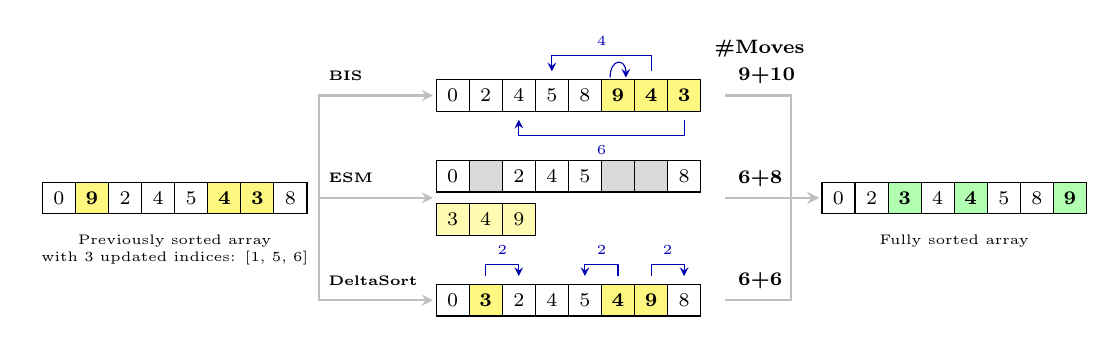
\begin{tikzpicture}[
    cell/.style={draw, minimum width=0.42cm, minimum height=0.4cm, font=\scriptsize},
    cellup/.style={cell, fill=yellow!50, font=\scriptsize\bfseries},
    cellgreen/.style={cell, fill=green!30, font=\scriptsize\bfseries},
    cellgrey/.style={cell, fill=gray!30},
    extracted/.style={draw, minimum width=0.42cm, minimum height=0.4cm, font=\scriptsize, fill=yellow!30},
    arrow/.style={->, >=stealth, thick, gray!50},
    movearrow/.style={->, >=stealth, blue!70!black},
    algo/.style={font=\scriptsize\bfseries},
    movelabel/.style={font=\tiny, blue!70!black},
    totalmoves/.style={font=\tiny\bfseries, black!70},
]

\def\cellw{0.42}
\def\rowA{0.8}    % BIS row
\def\rowB{-0.5}   % ESM row  
\def\rowC{-1.8}   % DeltaSort row

\def\xI{-0.5}     % Input column (shifted left)
\def\xM{4.5}      % Middle column (algorithm-specific)
\def\xO{9.4}      % Output column (shifted right)

% ============================================================================
% FIRST COLUMN: Shared Input Array
% ============================================================================
% Input: 0 9 2 4 5 4 3 8 (centered vertically between the 3 algo rows)
\foreach \i/\v/\up in {0/0/0, 1/9/1, 2/2/0, 3/4/0, 4/5/0, 5/4/1, 6/3/1, 7/8/0} {
    \ifnum\up=1
        \node[cellup] (I\i) at (\xI + \i*\cellw, \rowB) {\v};
    \else
        \node[cell] (I\i) at (\xI + \i*\cellw, \rowB) {\v};
    \fi
}
% Label below input array
\node[font=\tiny, anchor=north, text width=3.5cm, align=center] at (\xI + 3.5*\cellw, \rowB - 0.35) {Previously sorted array\\ with 3 updated indices: [1, 5, 6]};

% ============================================================================
% SECOND COLUMN: Algorithm-specific processing with movements
% ============================================================================

% --- BIS: 0 + 4 + 6 = 10 moves ---
% Label placed beside horizontal arm
% After moving dirty values to end: 0 2 4 5 8 9 4 3
\foreach \i/\v/\up in {0/0/0, 1/2/0, 2/4/0, 3/5/0, 4/8/0, 5/9/1, 6/4/1, 7/3/1} {
    \ifnum\up=1
        \node[cellup] (bisM\i) at (\xM + \i*\cellw, \rowA) {\v};
    \else
        \node[cell] (bisM\i) at (\xM + \i*\cellw, \rowA) {\v};
    \fi
}
% Movement arrows outside array: 9->self (0), 4->idx3 (4), 3->idx2 (6)
% Self-loop: starts from top-left of cell, curves up and right, ends at top-right
\draw[movearrow] ([xshift=-0.1cm, yshift=0.02cm]bisM5.north) 
    .. controls ++(0, 0.25) and ++(0, 0.25) .. 
    ([xshift=0.1cm, yshift=0.02cm]bisM5.north) node[above, movelabel, yshift=0.05cm, xshift=-0.1cm] {};
% Arrow for 4: goes above to avoid overlap with 6
\draw[movearrow] ([yshift=0.1cm]bisM6.north) -- ([yshift=0.3cm]bisM6.north) -| ([yshift=0.1cm]bisM3.north) node[pos=0.25, above, movelabel] {4};
% Arrow for 6: goes below
\draw[movearrow] ([yshift=-0.1cm]bisM7.south) -- ([yshift=-0.3cm]bisM7.south) -| ([yshift=-0.1cm]bisM2.south) node[pos=0.25, below, movelabel] {6};

% --- ESM: 3 + 3 + 5 = 11 moves ---
% Label placed beside horizontal arm
% Array with grey cells where 9, 4, 3 were removed (indices 1, 5, 6)
% Original: 0 9 2 4 5 4 3 8 -> 0 _ 2 4 5 _ _ 8
% Vertically centered between main array and extracted array
\foreach \i/\v/\grey in {0/0/0, 1//1, 2/2/0, 3/4/0, 4/5/0, 5//1, 6//1, 7/8/0} {
    \ifnum\grey=1
        \node[cellgrey] (esmM\i) at (\xM + \i*\cellw, \rowB + 0.275) {\v};
    \else
        \node[cell] (esmM\i) at (\xM + \i*\cellw, \rowB + 0.275) {\v};
    \fi
}
% Extracted sorted: 3 4 9 (below, aligned at same start)
\foreach \i/\v in {0/3, 1/4, 2/9} {
    \node[extracted] (esmE\i) at (\xM + \i*\cellw, \rowB - 0.275) {\v};
}

% --- DeltaSort: 3 + 2 + 2 + 2 = 9 moves ---
% Label placed beside horizontal arm
% After sorting k values in place: 9 4 3 -> 3 4 9 at indices 1, 5, 6
\foreach \i/\v/\up in {0/0/0, 1/3/1, 2/2/0, 3/4/0, 4/5/0, 5/4/1, 6/9/1, 7/8/0} {
    \ifnum\up=1
        \node[cellup] (dsM\i) at (\xM + \i*\cellw, \rowC) {\v};
    \else
        \node[cell] (dsM\i) at (\xM + \i*\cellw, \rowC) {\v};
    \fi
}
% Movement arrows: index 1->2 (2), index 5->4 (2), index 6->7 (2) - all above array
\draw[movearrow] ([yshift=0.1cm]dsM1.north) -- ([yshift=0.25cm]dsM1.north) -| ([yshift=0.1cm]dsM2.north) node[pos=0.25, above, movelabel] {2};
\draw[movearrow] ([yshift=0.1cm]dsM5.north) -- ([yshift=0.25cm]dsM5.north) -| ([yshift=0.1cm]dsM4.north) node[pos=0.25, above, movelabel] {2};
\draw[movearrow] ([yshift=0.1cm]dsM6.north) -- ([yshift=0.25cm]dsM6.north) -| ([yshift=0.1cm]dsM7.north) node[pos=0.25, above, movelabel] {2};

% ============================================================================
% THIRD COLUMN: Shared Output Array
% ============================================================================
% Output: 0 2 3 4 4 5 8 9 (centered vertically)
% 3, 4, 9 colored green (the updated values in final position)
\foreach \i/\v/\green in {0/0/0, 1/2/0, 2/3/1, 3/4/0, 4/4/1, 5/5/0, 6/8/0, 7/9/1} {
    \ifnum\green=1
        \node[cellgreen] (O\i) at (\xO + \i*\cellw, \rowB) {\v};
    \else
        \node[cell] (O\i) at (\xO + \i*\cellw, \rowB) {\v};
    \fi
}
% Label below output array
\node[font=\tiny, anchor=north] at (\xO + 3.5*\cellw, \rowB - 0.35) {Fully sorted array};

% ============================================================================
% Connecting arrows between columns (orthogonal with 90-degree turns)
% ============================================================================
\def\arrowgap{0.25}
\def\arrayw{8*\cellw}
\def\labelx{2.8}

% Input -> Middle (fan out to 3 algorithms)
% Horizontal then vertical - turn point shifted left for longer horizontal arms
% Labels at fixed x position (left-aligned), black color, above arrows
\draw[arrow] (\xI + \arrayw + \arrowgap, \rowB) -- (2.8, \rowB) -- (2.8, \rowA) -- (\xM - \arrowgap, \rowA);
\node[font=\scriptsize\bfseries\tiny, black, anchor=west] at (\labelx, \rowA + 0.25) {BIS};
\draw[arrow] (\xI + \arrayw + \arrowgap, \rowB) -- (\xM - \arrowgap, \rowB);
\node[font=\scriptsize\bfseries\tiny, black, anchor=west] at (\labelx, \rowB + 0.25) {ESM};
\draw[arrow] (\xI + \arrayw + \arrowgap, \rowB) -- (2.8, \rowB) -- (2.8, \rowC) -- (\xM - \arrowgap, \rowC);
\node[font=\scriptsize\bfseries\tiny, black, anchor=west] at (\labelx, \rowC + 0.25) {DeltaSort};
% Middle -> Output (fan in from 3 algorithms)
% Horizontal then vertical - consistent with column 1->2 arrows
% Labels showing total moves for each algorithm
\node[black, anchor=west] at (7.7, \rowA + 0.6) {\scriptsize\bfseries \#Moves};
\draw[arrow] (\xM + \arrayw + 0.1, \rowA) -- (8.8, \rowA) -- (8.8, \rowB) -- (\xO - \arrowgap, \rowB);
\node[black, anchor=west] at (8.0, \rowA + 0.25) {\scriptsize\bfseries 9+10};
\draw[arrow] (\xM + \arrayw + 0.1, \rowB) -- (\xO - \arrowgap, \rowB);
\node[black, anchor=west] at (8.0, \rowB + 0.25) {\scriptsize\bfseries 6+8};
\draw[arrow] (\xM + \arrayw + 0.1, \rowC) -- (8.8, \rowC) -- (8.8, \rowB) -- (\xO - \arrowgap, \rowB);
\node[black, anchor=west] at (8.0, \rowC + 0.25) {\scriptsize\bfseries 6+6};
\end{tikzpicture}
\caption{Data movement comparison for 3 updated values (yellow). BIS first uses 9 moves to shift updated values to the end (since insertion requires a fully sorted prefix), then 10 (0+4+6) moves to insert each into the sorted prefix. ESM uses 6 moves to sort the extracted values, then writes all 8 values to produce the merged output. DeltaSort uses 6 moves to sort updated values, then just 6 (2+2+2) moves to place each value correctly within its segment (see~\defref{def:segment}), \textbf{without having to form a fully sorted prefix upfront} like BIS.}
\label{fig:algorithm-comparison}
\end{figure}
